%%% Local Variables:
%%% mode: latex
%%% TeX-master: "report_main"
%%% End:
\section{Part 4 -- State estimation}
This section consists of the development of an observer to estimate the
nonmeasured angular velocities.
%
\subsection{Problem 1}
By describing the system in \cref{eq:linearized EoM} in the following
state-space form
%
\begin{align}
  \begin{split}
    \dot{\bm{x}} &= \bm{Ax} + \bm{Bu} \\
    \bm{y} &= \bm{Cx}
  \end{split}
\end{align}
%
where  $\bm{A}$, $\bm{B}$ and $\bm{C}$ are matrices. The state -,
input - and output vector are given by
%
\begin{equation}
  \label{eq:state_space_vectors}
  \bm{x} =
  \begin{bmatrix}
    \tilde{p} \\
    \dot{\tilde{p}} \\
    \tilde{e} \\
    \dot{\tilde{e}} \\
    \tilde{\lambda} \\
    \dot{\tilde{\lambda}} \\
  \end{bmatrix}
  , \quad \bm{u} =
  \begin{bmatrix}
    \tilde{V_s} \\
    \tilde{V_d} \\
  \end{bmatrix}
  \quad \text{and} \quad \bm{y} =
  \begin{bmatrix}
    \tilde{p} \\
    \tilde{e} \\
    \tilde{\lambda}\\
  \end{bmatrix}
\end{equation}
%
This gives the following $\bm{A}$, $\bm{B}$ and $\bm{C}$ matrices
%
\begin{equation}
  \label{eq:state_space_A_B_C}
  \bm{A} =
  \begin{bmatrix}
    0 & 1 & 0 & 0 & 0 & 0 \\
    0 & 0 & 0 & 0 & 0 & 0 \\
    0 & 0 & 0 & 1 & 0 & 0 \\
    0 & 0 & 0 & 0 & 0 & 0 \\
    0 & 0 & 0 & 0 & 0 & 1 \\
    K_3 & 0 & 0 & 0 & 0 & 0 \\
  \end{bmatrix}
  , \quad \bm{B} =
  \begin{bmatrix}
    0 & 0 \\
    0 & K_1 \\
    0 & 0 \\
    K_2 & 0 \\
    0 & 0 \\
    0 & 0 \\
  \end{bmatrix}
  \quad \text{and} \quad \bm{C} =
  \begin{bmatrix}
    1 & 0 & 0 & 0 & 0 & 0 \\
    0 & 0 & 1 & 0 & 0 & 0 \\
    0 & 0 & 0 & 0 & 1 & 0 \\
  \end{bmatrix}
\end{equation}
%
Where $K_1$, $K_2$ and $K_3$ are given by \cref{eq:linearized EoM}.
%
\subsection{Problem 2}
The observer matrix can be used. For a 6 state system, it is define by:
\begin{equation}
  \bm{\mathcal{O}} =
  \begin{bmatrix}
    \bm{C} \\
    \bm{CA} \\
    \bm{C*A^2} \\
    \bm{C*A^3} \\
    \bm{C*A^4} \\
    \bm{C*A^5} \\
  \end{bmatrix} \\
\end{equation}
This can be calculated using MATLAB's $obsv(\bm{A},\bm{C})$
function. The resulting 18x6 matrix has rank 6, thereby full rank.
%
% &=\begin{bmatrix}
%   1 & 0 & 0 & 0 & 0 & 0 \\
%   0 & 0 & 1 & 0 & 0 & 0 \\
%   0 & 0 & 0 & 0 & 1 & 0 \\
%   0 & 1 & 0 & 0 & 0 & 0 \\
%   0 & 0 & 0 & 1 & 0 & 0 \\
%   0 & 0 & 0 & 0 & 0 & 1
% \end{bmatrix}
% \end{align*}
It has full rank, and the system is therefore fully observable.

The observer gain matrix $\bm{L}$ is to be set in such a way that the
poles of the observer is faster than the system, in order to drive the
error to zero.
\begin{figure}[H]
  \caption{ illustrating how to place poles during state, or estimated
    state feedback, on a semi-circle with the same radius, within the
    region shown.}
  \label{fig:pole_placement}
  \begin{center}
    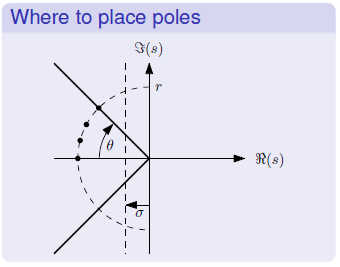
\includegraphics[width=0.5\textwidth]{images/pole_placement}
  \end{center}
\end{figure}
\todo[inline]{Finn navnene på theta og sigma i forhold til regtek}The
poles of the observer must be placed as in
\cref{fig:pole_placement}. The real value of our poles must be larger
than $\sigma$, which for the observer is the value of the largest real
value of the controlled systems poles. This way, all of the linear
observers poles are faster than the controlled system. $\theta$ is the
biggest angle of our observer poles. If this is too large, we will get
too much of an underdamped system and too much of an
overshoot. However, if the radius is too large, undesired high
frequency noise from the measurements becomes amplified to unwanted
levels.

We chose $\theta = 15$, and $r$ as 50 times the maximum length of the
controlled systems poles.

The observer itself has the state space formulation:

\begin{equation*}
  \dot{\hat{\bm{x}}} = \bm{A}\hat{\bm{x}}+\bm{B}\bm{u} + \bm{L}(\bm{y}
  - \bm{C}\hat{\bm{x}})
\end{equation*}
\begin{align*}
  \dot{\bm{e}} &= \dot{\bm{\tilde{x}}} - \dot{\hat{\bm{x}}} \\
							 &= \bm{Ax} + \bm{Bu} - \bm{A}\hat{\bm{x}} - \bm{Bu} - \bm{L}(\bm{y}- \bm{C}\hat{\bm{x}}) \\
							 &= \bm{A}(\bm{x} - \hat{\bm{x}}) - \bm{L}(\bm{C}\bm{x}- \bm{C}\hat{\bm{x}}) \\
							 &= \bm{Ae} - \bm{LCe} \\
\end{align*}
Meaning our error has the state space formulation:
\begin{equation}
	\dot{\bm{e}} = (\bm{A} - \bm{LC})\bm{e}
\end{equation}
As previously stated, we need this error to converge to zero by placing the poles of this state space formulation such that they are faster than the poles of the system itself. The poles of this state space system can be placed arbitrarily because $\{\bm{A},\bm{C}\}$ is observable:
\begin{equation*}
det(\lambda\bm{I} - \bm{A} +\bm{LC}) = 0
\end{equation*}
For this equation, $\lambda$ are the values that solves the equation, and also the poles of the observer. By choosing values for $\lambda$, an $\bm{L}$ emerges in order to make the determinant equal to zero. The matlab function $place$ places the poles as desired for us: $\bm{L} = place(\bm{A}^T,\bm{C}^T,\bm{\lambda})^T$, where $\bm{\lambda}$ is the vector of the observer poles in this instance.

\subsection{Problem 3}
When only $\tilde{e}$ and $\tilde{\lambda}$ are measured, the output
matrix $\bm{C}$ becomes:
$\begin{bmatrix}
  0 & 0 & 1 & 0 & 0 & 0 \\
  0 & 0 & 0 & 0 & 1 & 0
\end{bmatrix}$.
The observer matrix, found through $obsv(\bm{A},\bm{C})$ is a 12x6
matrix with rank 6. Therefore, it is observable.

However, when only $\tilde{p}$ and $\tilde{e}$ are measured, the
output matrix $\bm{C}$ becomes:
$\begin{bmatrix}
  1 & 0 & 0 & 0 & 0 & 0 \\
  0 & 0 & 1 & 0 & 0 & 0
\end{bmatrix}$.
The observer matrix, found through $obsv(\bm{A},\bm{C})$ is a 12x6
matrix with rank 4. Therefore, it is not observable.
% \begin{equation}
%   \bm{\mathcal{O}} =
%   \begin{bmatrix}
%     0 & 0 & 1 & 0 & 0 & 0 \\
%     0 & 0 & 0 & 0 & 1 & 0 \\
%     0 & 0 & 0 & 0 & 0 & 0 \\
%     0 & 1 & 0 & 0 & 0 & 0 \\
%     0 & 0 & 0 & 1 & 0 & 0 \\
%     0 & 0 & 0 & 0 & 0 & 1
%   \end{bmatrix}
% \end{equation}
